\documentclass{article}

% Symbols
\usepackage{amsfonts, amsthm}
\usepackage{upgreek}
\usepackage{physics}
\usepackage{cancel}
\usepackage{amssymb, latexsym, amsmath}
\usepackage{import}

%Algorithms
\usepackage[ruled,lined,linesnumbered,commentsnumbered]{algorithm2e}

%% Identación
\setlength{\parindent}{0cm}

% Código
\newcommand{\code}[1]{\textcolor{white!25!black}{\texttt{#1}}}
\usepackage{listings}

%AMS
\usepackage{amsthm}
\newtheorem{algo-thm}{Algoritmo}

% Graphics
\usepackage{graphicx}
\usepackage{pgf}

% Margins
\addtolength{\voffset}{-1.5cm}
\addtolength{\hoffset}{-1.5cm}
\addtolength{\textwidth}{3cm}
\addtolength{\textheight}{3cm}

%Header-Footer
\usepackage{fancyhdr}
\renewcommand{\headrulewidth}{1pt}

\newcommand{\set}[1]{
  \left\{ #1 \right\}
}

\footskip = 50pt
\renewcommand{\headrulewidth}{1pt}

\pagestyle{fancyplain}

\begin{document}
\title{UNIVERSIDAD NACIONAL AUT\'ONOMA DE M\'EXICO\\ Facultad de Ciencias}
\author{Integrantes:\\
  Diego Angel Rosas Franco\\
  Adri\'an Aguilera Moreno\\
  Marco Antonio Rivera Silva}
\date{}
\maketitle
\begin{center}
  
\includegraphics[scale=0.20]{../Portada/Portada}\\[0.4cm]
  \Large
  \bf{Modelado y programación}
  \normalsize
\end{center}
\newpage
\fancyhead[r]{ Modelado y programación 2022-2}


\section*{\LARGE{Práctica 4}}

Menciona los principios de diseño esenciales de los patrones Factory, Abstract Factory y Builder.
Menciona una desventaja de cada patrón.

\subsubsection*{Factory}
Principios de diseño :
\newcommand{\localtextbulletone}{\textcolor{black}{\raisebox{.45ex}{\rule{.6ex}{.6ex}}}}
\renewcommand{\labelitemi}{\localtextbulletone}
\begin{itemize}
\item Esta abierto al cambio pero no a la modificación, es decir que te permiten añadir
  clases nuevas sin que el código tenga que cambiar de ninguna manera.
\item Si una de las clases, que no sea la principal y que a su vez forme parte del patrón,
  no funciona de manera correcta, esta no afecta a las demás, pues es esta quién depende de
  alguna otra y no al réves.
\item Ordena la herencia en las clases.
\end{itemize}
Desventajas:
\begin{itemize}
\item No es el patrón más óptimo para complejidad en espacio.
\item Se necesitan muchas clases para concretar el patrón, y cada vez que se quiera extender,
  entonces se agregan más clases.
\item Cada vez que se necesita anexar más partes de código le agregamos complejidad al diseño,
  esto no permite que sea tan fácil.
\end{itemize}
\subsubsection*{Abstract Factory}
Principios de diseño :
\begin{itemize}
\item Encapsula la responsabilidades de los objetos.
\item Hace intercambiables compartamientos que ya dependen de alguna implementación del patrón
  \code{abstract factory}.
\item Los comportamientos en una familia dada son compatibles entre sí.
\item Se puede mover el código de creación de productos a un solo lugar,
  haciendo que el código sea más fácil de mantener.
\item Es abierto al cambio y cerrado a la modificación
\end{itemize}
Desventajas:
\begin{itemize}
\item Cada vez que necesitemos anexar más comportamientos o clases, se necesitará una nueva
  interfaz (en caso de no poder depender de alguna ya existente) e implementar cada método
  en esta.
\item Crece en complejidad en espacio.
\item Hace más complejo el diseño del código.
\end{itemize}
\subsubsection*{Builder}
Principios de diseño :
\begin{itemize}
\item El código puede ser reutilizable, o ser extendido y modificado de manera significativa,
  esto simplifica el proceso de extensión cuando el comportamiento a anexar tiene similitudes
  con los ya existentes.
\item Puedes construir objetos paso a paso.
\item A menudo se usa para construir estructuras compuestas.
\end{itemize}
Desventajas:
\begin{itemize}
\item El diseño del código se vuelve complejo.
\item Aumenta la complejidad en espacio.
\end{itemize}


\subsection*{Instrucciones de instalación, compilación y ejecución.}
Se dará por hecho que el usuario sabe moverse en terminal.\\

\subsubsection*{Requerimientos previos:}
\begin{itemize}
\item[-] Se debe contar con Java en su computadora. De preferencia la versión más reciente.
\end{itemize}

\subsubsection*{Ejecución del proyecto:}
\begin{itemize}
\item[-] Si está leyendo esto significa que desempaquetó con éxito el proyecto.
\item[-] Abra su terminal y diríjase a la ruta donde desempaquetó el proyecto.
\item[-] Una vez estando en la ruta \code{Practica04\_NullPointerException}, diríjase a

  \code{Practica04\_NullPointerException/src/fciencias/modelado/}
\item[-] Ejecute: “\code{javac Práctica04.java}”, esto generará los .class del proyecto.
\item[-] Ejecute: “\code{java Práctica04}”, esto ejecutará el proyecto mostrándole el menú solicitado para la practica.
\end{itemize}

\newpage
\subsection*{Diagrama UML:}
%\begin{center}
%  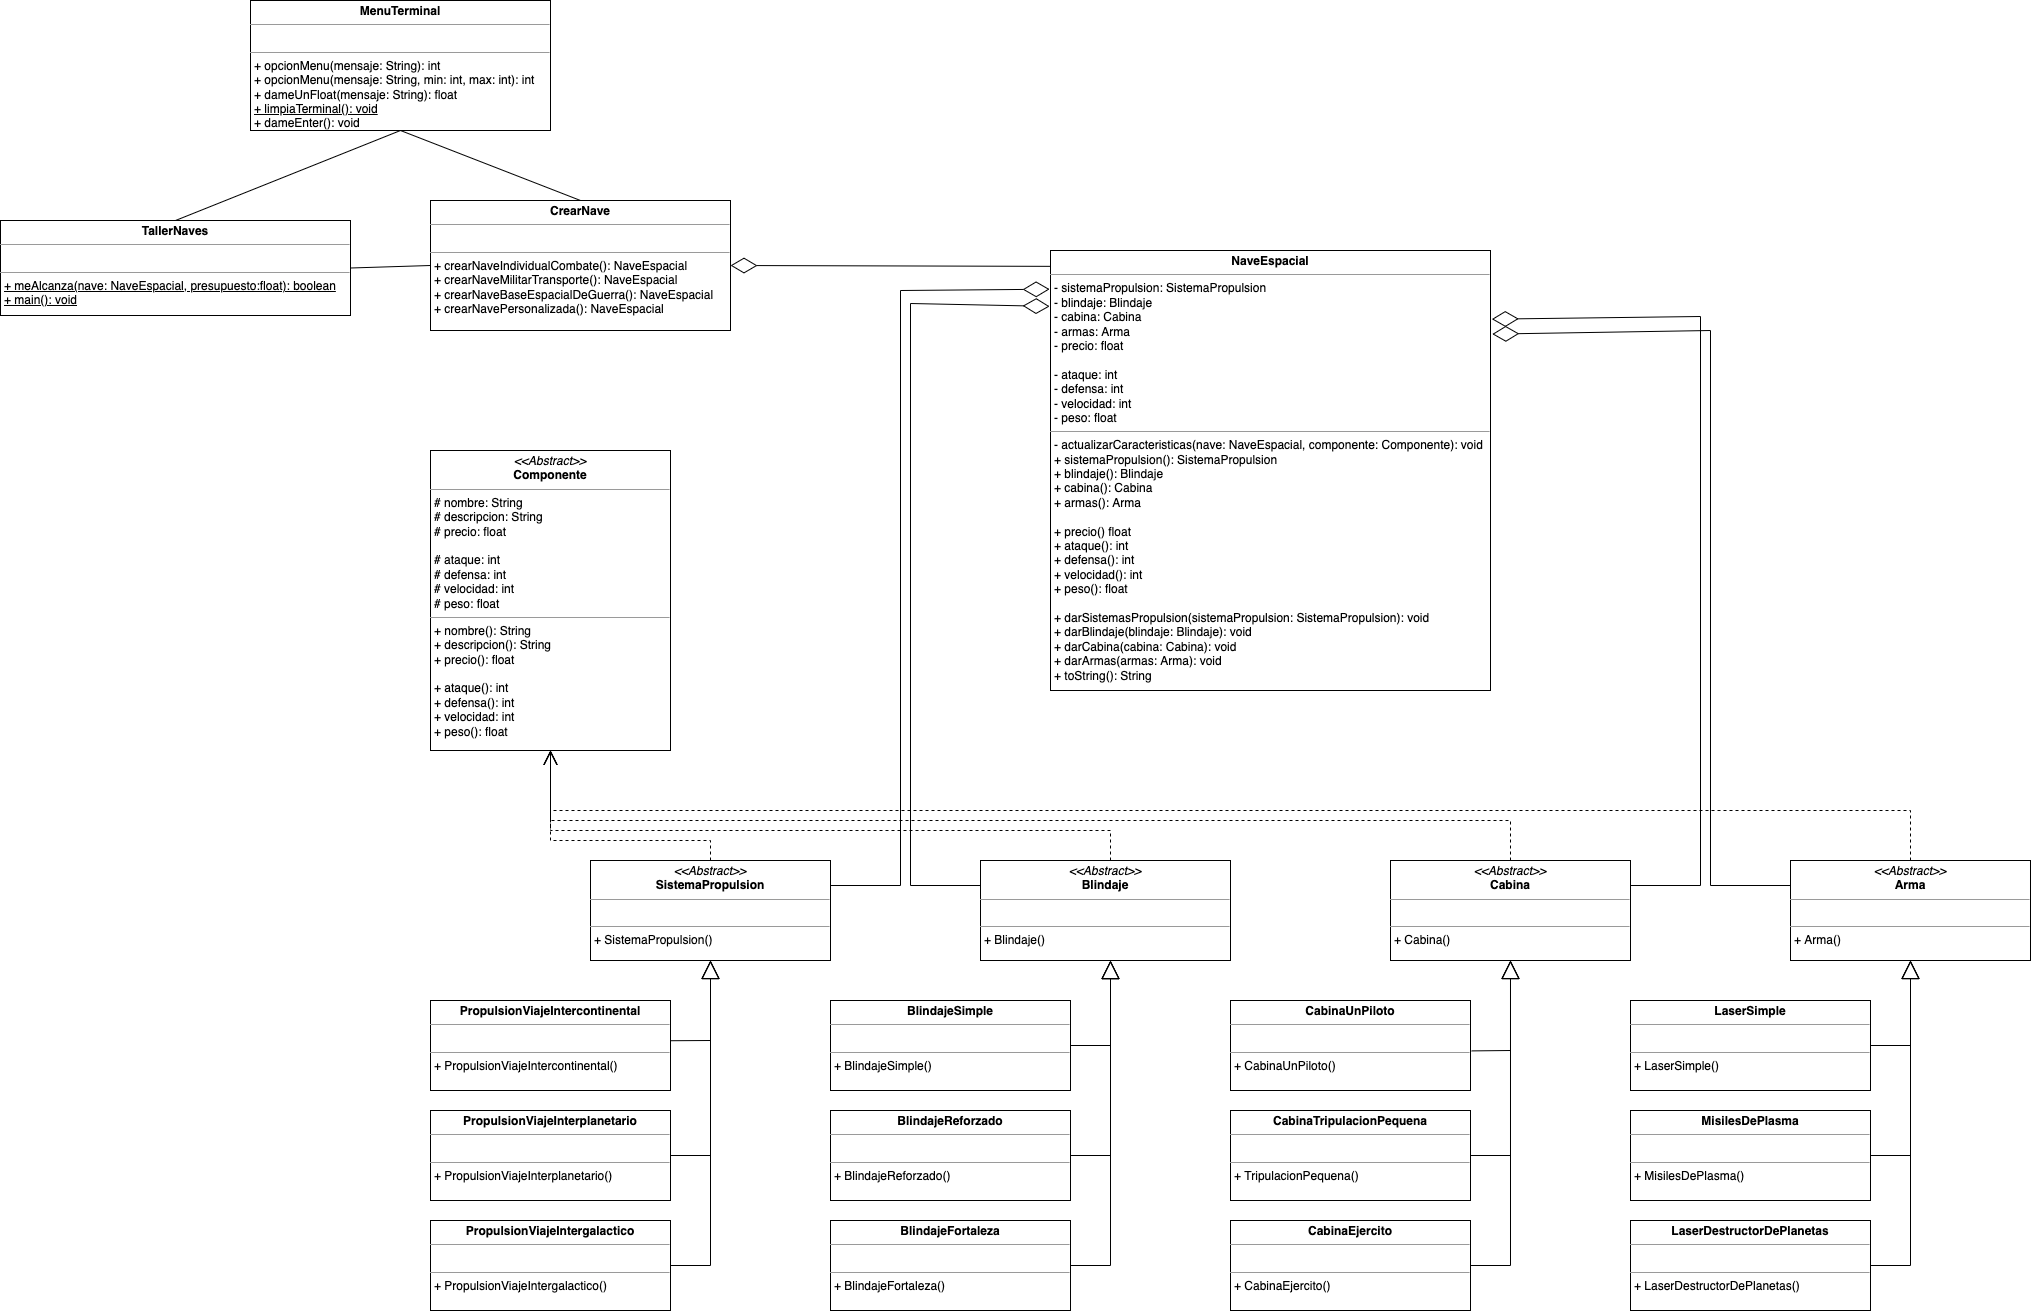
\includegraphics[scale=0.16]{./Practica04UML.png}
%\end{center}
\end{document}
